\documentclass{beamer}
\usepackage[utf8]{inputenc}
\usepackage[T1]{fontenc}
\title{Machine Learning for spoken commands classification}
\author{Thomas Marquet}

\usetheme{UniKlu}

\begin{document}
	
	\begin{frame}
		\titlepage
	\end{frame}
	
	\begin{frame}{Summary}
		\tableofcontents[]
	\end{frame}	
	
	\begin{frame}{Motivation} 
		\begin{itemize}
		    \item First step to make it's own Jarvis at home (or at least a less than intelligent coffee machine)
		    \item It can be used afterwards to be attacked in the context of my PhD Thesis
		\end{itemize}
		
	\end{frame}

	\begin{frame}{Learning Task} 
        The Learning task is about the classification of 20 one word spoken commands plus being able to recognize unlabeled words and silence. Therefore the output is on 22 labels.
        \vspace{5mm}
        The following words are the targets :
        \begin{figure}
            \centering
            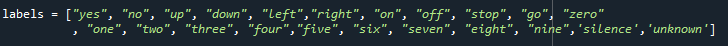
\includegraphics[width=1\textwidth]{pics/labels.PNG}

        \end{figure}
        
        
        \vspace{5mm}
        Those words are used to represent the unknown label :
        \begin{figure}
            \centering
            
\includegraphics[width=1\textwidth]{pics/unknown_labels.PNG}

        \end{figure}        
        
	\end{frame}

	\begin{frame}{Related Work} 

	\end{frame}
	
	\begin{frame}{Data Analysis} 

	\end{frame}
	
	\begin{frame}{Model : MLP}

	\end{frame}

	\begin{frame}{Model : CNN}

	\end{frame}
	\begin{frame}{Model : Small CNN}

	\end{frame}	
	
	\begin{frame}{Model : LSTM}

	\end{frame}	
	
	\begin{frame}{Model : LSTM + convolutions}

	\end{frame}

	\begin{frame}{Live Demo}

	\end{frame}	
	
	\begin{frame}{Conclusion}

	\end{frame}		
\end{document}